\documentclass[12pt]{article}

\usepackage[margin = 1in]{geometry}
\usepackage{graphicx}              
\usepackage{amsmath}               
\usepackage{amsfonts}              
\usepackage{amsthm}                
\usepackage{amssymb}
\usepackage{mathrsfs}
\usepackage{url}
\usepackage{subfig}
\usepackage{xfrac}
\usepackage[sectionbib]{chapterbib}
\usepackage{hyperref}
\usepackage{tikz}
\usetikzlibrary{positioning}
\usetikzlibrary{calc}
\usepackage{algorithmic}


\hypersetup{
	unicode=true,
	colorlinks=true,
	citecolor=black,
	filecolor=black,
	linkcolor=black,
	urlcolor=black,
	pdfstartview={FitH},
}

% theorem environments
\theoremstyle{plain}
\newtheorem{theorem}{Theorem}
\newtheorem{lemma}[theorem]{Lemma}
\newtheorem{corollary}[theorem]{Corollary}
\newtheorem{proposition}[theorem]{Proposition}
\theoremstyle{definition}
\newtheorem{definition}[theorem]{Definition}
\newtheorem{conjecture}[theorem]{Conjecture}
\newtheorem{example}[theorem]{Example}
\newtheorem*{remark}{Remark}
\newtheorem*{note}{Note}


\renewcommand{\algorithmicrequire}{\textbf{Input:}}
\renewcommand{\algorithmicensure}{\textbf{Output:}}
\algsetup{linenodelimiter=.}

\newcommand{\wrt}{\vdash} 
\newcommand{\ang}[1]{\langle#1\rangle}
\newcommand{\abs}[1]{\left\vert#1\right\vert}
\newcommand{\dual}[1]{\overline{#1}}
\newcommand{\mapsfrom}{\ensuremath{\reflectbox{$\mapsto$}}}
\newcommand{\tildO}{\tilde{O}}
% roman numerals
\newcommand{\romnum}[1]{\romannumeral #1}
\newcommand{\Romnum}[1]{\uppercase\expandafter{\romannumeral #1}}
\newcommand{\todo}[1]{\textcolor{red}{TODO: #1}}


\DeclareMathOperator{\fieldchar}{char} % characteristic of a field
\DeclareMathOperator{\ringofend}{End} % endomorphism ring
\DeclareMathOperator{\trace}{tr} % trace of a mtrix
\DeclareMathOperator{\gal}{Gal} % Galois group
\DeclareMathOperator{\order}{ord} % order of an element
\DeclareMathOperator{\lcm}{lcm} % least common multiple
\DeclareMathOperator{\divisor}{div} % divisor on a curve
\DeclareMathOperator{\supp}{supp} % support of a divisor
\DeclareMathOperator{\norm}{N} % norm
\DeclareMathOperator{\Res}{Res}
\DeclareMathOperator{\Aut}{Aut}

\def\Q{\ensuremath{\mathbb{Q}}}
\def\N{\ensuremath{\mathbb{N}}}
\def\R{\ensuremath{\mathbb{R}}}
\def\Z{\ensuremath{\mathbb{Z}}}
\def\F{\ensuremath{\mathbb{F}}}
\def\H{\ensuremath{\mathbb{H}}}
\def\K{\ensuremath{\mathbb{K}}}
\def\L{\ensuremath{\mathbb{L}}}
\def\A{\ensuremath{\mathbb{A}}}
\def\B{\ensuremath{\mathbb{B}}}
\def\MM{\ensuremath{\mathsf{M}}}
\def\II{\ensuremath{\mathsf{I}}}
\def\QQ{\ensuremath{\mathsf{Q}}}
\def\CC{\ensuremath{\mathsf{C}}}
\def\RR{\ensuremath{\mathsf{R}}}
\def\AA{\ensuremath{\mathsf{A}}}
\def\va{\ensuremath{\mathsf{a}}}
\def\vy{\ensuremath{\mathsf{y}}}
\def\vu{\ensuremath{\mathsf{u}}}
\def\vb{\ensuremath{\mathsf{b}}}
\def\vc{\ensuremath{\mathsf{c}}}
\def\mul{\ensuremath{\mathsf{mul}}}
\def\rem{\ensuremath{\mathsf{rem}}}
\def\cat{\ensuremath{\mathsf{cat}}}
\def\coeff{\ensuremath{\mathsf{coefficient}}}
\def\mulmod{\ensuremath{\mathsf{mulmod}}}
\def\rev{\ensuremath{\mathsf{rev}}}
\def\x{\ensuremath{\mathbf{x}}}
\def\uu{\ensuremath{\mathbf{U}}}
\def\bb{\ensuremath{\mathbf{B}}}
\def\bxi{\boldsymbol{\xi}}
\def\bupsilon{\boldsymbol{\upsilon}}
\def\bzeta{\boldsymbol{\zeta}}
\def\blambda{\boldsymbol{\lambda}}


% allow algorithms to split over multiple pages
\makeatletter
\newcounter{algorithm}
\setcounter{algorithm}{0}
\renewcommand{\thealgorithm}{\arabic{algorithm}}
\def\algorithm{\@ifnextchar[{\@algorithma}{\@algorithmb}}
\def\@algorithma[#1]{%
	\refstepcounter{algorithm}
	\trivlist
	\leftmargin\z@
	\itemindent\z@
	\labelsep\z@
	\item[\parbox{\columnwidth}{%
		\hrule
		\hrule
		\noindent\strut\textbf{Algorithm \thealgorithm} #1
		\hrule
	}]\hfil\vskip0em%
}
\def\@algorithmb{\@algorithma[]}
\def\endalgorithm{\hfil\vskip-1em\hrule\endtrivlist}
\makeatother


\title{Computing isomorphisms and embeddings of finite fields}
\author{Ludovic Brieulle, Luca De Feo, Javad Doliskani,\\ Jean Pierre
  Flori and Éric Schost}


\begin{document}

\maketitle
\begin{abstract}
  Let $\F_q$ be a finite field.  The finite field isomorphism problem
  asks, given two irreducible polynomials $f,g$ in $\F_q[X]$ with
  $\deg f$ dividing $\deg g$, to compute an explicit description of a
  field embedding of $\F_q[X]/f$ into $\F_q[X]/g$. When $\deg f = \deg
  g$, this is also known as the isomorphism problem.
  
  We review classical algorithms for the two problems, and compare
  their asymptotic complexities. We also propose new improvements and
  generalizations to the algorithms, implement them, and compare them
  with the state of the art.
\end{abstract}

%%%%%%%%%%%%%%%%%%%%%%%%%%%%%%%%%%
%%%%%%%%%%%%%%%%%%%%%%%%%%%%%%%%%%

\section{Introduction}

Let $q$ be a prime power and let $\F_q$ be a field with $q$
elements. Let $f$ and $g$ be irreducible polynomials in $\F_q[X]$,
with $\deg f$ dividing $\deg g$. Define $k=\F_q[X]/f$ and
$K=\F_q[X]/g$, then there is an embedding $\varphi:k\hookrightarrow
K$, unique up to $\F_q$-automorphisms of $k$. The goal of this paper
is to describe algorithms to efficiently represent and evaluate one
such embedding.

\todo{Motivation, previous work.}

All the algorithms we are aware of, split the embedding problem in two
sub-problems:
\begin{enumerate}
\item Determine elements $\alpha\in k$ and $\beta\in K$ such that
  $k=\F_q[\alpha]$, $K=\F_q[\beta]$, and such that there exists an
  embedding $\varphi$ mapping $\alpha\mapsto\beta$. We refer to this
  problem as the \emph{Embedding description}.
\item Given elements $\alpha$ and $\beta$ as above, given $\gamma\in
  k$ and $\delta\in K$, solve the following problems:
  \begin{itemize}
  \item Compute $\varphi(\gamma)\in K$.
  \item Test if $\delta\in\varphi(k)$.
  \item If $\delta\in\varphi(k)$, compute $\varphi^{-1}(\delta)\in K$.
  \end{itemize}
  We refer collectively to these problems as the \emph{Embedding
    evaluation}.
\end{enumerate}

\paragraph{Complexity notation} We measure all complexities in number
of operations $+$, $\times$, $\div$ in $\F_q$. We write $\MM(n)$ for
the cost of multiplying two polynomials in $\F_q[X]$ of degree at most
$n$.


\subsection{Naive algorithms}

\todo{Describe polynomial factorization}

\todo{Describe linear algebra}


%%%%%%%%%%%%%%%%%%%%%%%%%%%%%%%%%%
%%%%%%%%%%%%%%%%%%%%%%%%%%%%%%%%%%

\part{Embedding description}

%%%%%%%%%%%%%%%%%%%%%%%%%%%%%%%%%%

\section{Kummer-type algorithms}

In this section we review what we call \textit{Kummer-type} approaches to the isomorphism problem. 
We briefly review the works of Lenstra \cite{LenstraJr91}, and Allombert \cite{Allombert02}, and at 
the end we give a variant of these algorithms with a significantly lower running time complexity.

Let $F$ be an extension of degree $r$ of $E = \F_q$. In \cite{LenstraJr91}, Lenstra proves that 
given two finite fields of the same size, there exists a deterministic polynomial time algorithm 
that finds an isomorphism between them. The focus of the paper is on the theoretical construction 
of the isomorphism, and no rigorous complexity analysis is presented. However, since there is an 
explicit assumption of using linear algebra in the paper, a rough analysis of the algorithm yields 
an estimate of $O(r^3)$ operations in $E$. The idea of the algorithm is as follows. First, if 
the extension degree is equal to the charactristic the Artin-Schreier theory is used. Therefore, we 
assume $p \ne r$.

Let $E[\zeta]$ denote the ring extension $E[X] / \Phi_r(X)$ where $\Phi_r$ is the $r$th cyclotomic 
polynomial. Also let $\Delta$ denote the group of automorphisms $\Aut(E[\zeta]/E)$. Then we have 
$E[\zeta]^\Delta = E$. Let $E[\zeta][c^{1/r}]$ denote the quotient $E[\zeta][Y]/\ang{Y^r - c}$ such 
that $c^{1/r}$ is the residue class of $Y$. For a given element $c \in T_E$, where $T_E$ is the 
Teichm\"{u}ller subgroup \footnote{See the reference for details.} of $E[\zeta]$, the action of 
$\Delta$ can be extended over the ring $E[\zeta][c^{1/r}]$ by sending $c^{1/r}$ to powers 
$(c^{1/r})^\ell$ for certain integers $\ell$. If $c_1, c_2 \in T_E$ have the same order then we can 
find an isomorphism $E[\zeta][c_1^{1/r}] \cong E[\zeta][c_2^{1/r}]$ that is identity on $E[\zeta]$ 
and preserves the action of $\Delta$. In fact since $c_1$ and $c_2$ both generate the same 
subgroups, there is an integer $j > 0$ such that $c_1 = c_2^j$, and the isomorphism is given by
\[
\begin{array}{lrll}
	\psi: & E[\zeta][c_1^{1/r}] & \rightarrow & E[\zeta][c_2^{1/r}] \\
	& c_1^{1/r} & \mapsto & (c_2^{1/r})^j
\end{array}
\]
If $c$ is a generator of $T_E$ then we can show that $E[\zeta][c^{1/r}]^\Delta$ is a field 
extension of $E$ of degree $r$. Also, we can find an element $\gamma \in F[\zeta]$ such that $c 
= \gamma^r$ belongs to $E[\zeta]^*$ and	generates $T_E$. This gives an isomorphism $F[\zeta] \cong 
E[\zeta][c^{1/r}]$ that is identity on $E[\zeta]$, sends $\gamma$ to $c^{1/r}$, and preserve the 
action of $\Delta$. From this isomorphism we get the induced isomorphism $F \cong 
E[\zeta][c^{1/r}]^\Delta$. Therefore, given extensions $F_1, F_2$ of $E$ of degree $r$, we have 
built a chain
\begin{equation*}
	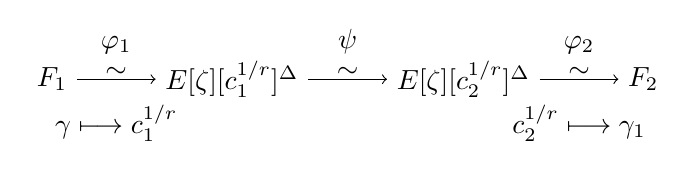
\begin{tikzpicture}
		\node (Ec1) {$E[\zeta][c_1^{1/r}]^\Delta$};
		\node[right = of Ec1] (Ec2) {$E[\zeta][c_2^{1/r}]^\Delta$};
		\node[left = of Ec1] (F1) {$F_1$};
		\node[right = of Ec2] (F2) {$F_2$};
		\draw[->] (F1) edge node[above, inner sep=0.5pt] {$\sim$} node[above = 3mm, inner 
		sep=0.5pt] {$\varphi_1$} node[below = 3mm, inner sep=0.5pt] {$\gamma \longmapsto 
		c_1^{1/r}$} (Ec1);
		\draw[->] (Ec1) edge node[above, inner sep=0.5pt] {$\sim$} node[above = 3mm, inner 
		sep=0.5pt] {$ \psi $} (Ec2);
		\draw[->] (Ec2) edge node[above, inner sep=0.5pt] {$\sim$} node[above = 3mm, inner 
		sep=0.5pt] {$ \varphi_2 $} node[below = 3mm, inner sep=0.5pt] {$c_2^{1/r} \longmapsto 
		\gamma_1$} (F2);
	\end{tikzpicture}
\end{equation*}
of isomorphisms. The following algorithm summarizes the process.
\begin{algorithm}[Lesntra]
	\begin{algorithmic}[1]
		\REQUIRE Field extensions $F_1, F_2$ of $E$ of degree $r$
		\ENSURE An isomorphism $\F_1 \xrightarrow{\sim} F_2$
		\STATE find a generator $c_i$ of $T_{F_i}$ for $i = 1, 2$
		\STATE find isomorphisms $\varphi_i: F_i \xrightarrow{\sim} E[\zeta][c_i^{1/r}]^\Delta$ for 
		$i = 1, 2$
		\STATE compute the integer $j$ such that $c_1 = c_2^j$
		\STATE build the isomorphism $\psi: E[\zeta][c_1^{1/r}]^\Delta \xrightarrow{\sim} 
		E[\zeta][c_2^{1/r}]^\Delta$
		\RETURN $\varphi_2 \circ \psi \circ \varphi_1$
	\end{algorithmic}
\end{algorithm}
A more careful look at the above approach suggests a trade-off between determinism and 
simplicity/practicality. For example, one can replace the ring extension $E[\zeta]$ with the field 
extension $E[\zeta] = E[X] / \ang{g}$ where $g$ is an irreducible factor of $\Phi_r$. This makes 
things simpler and more practical at the cost of factoring $\Phi_r$ which of course introduces 
indeterminism if one chose to use efficient factoring algorithms.

Alombert's approach is more or less the same as above with more focus on implementation. The idea 
of the algorithm is to cyclotomic field extensions which in turn allows the explicit use of Hilbert 
90 Theorem to find elements $\alpha_1 \in F_1[\zeta]$, and $\alpha_2 \in F_2[\zeta]$. Then $b = 
\alpha_1^r / \alpha_2^r$ is an $r$th power in $E[\zeta]$ from which $b^{1/r}$ can be computed using 
a root extraction algorithm. The isomorphism $F_1[\zeta] \xrightarrow{\sim} F_2[\zeta]$ is then 
given by $\alpha_1 \mapsto b^{1/r}\alpha_2$. Although again no rigorous complexity analysis is 
presented, one can easily see that the dominant cost of this algorithm is solving Hilbert 90 which 
is done using linear algebra. Therefore, the algorithm performs $O(n^{\omega + 1})$ many operations 
in $E$.


\subsection{Fast variant}
In this section we give an asymptotically faster and more practical version of the above 
algorithms. We replace linear algebra with polynomial arithmetic, and use a trace-like computation 
technique to solve Hilbert 90. 

An overview of the construction is as follows. For simplicity we 
work over the prime field $\F_p$ for a given prime $p$. Suppose we are given extensions $F_1, F_2$ 
of $\F_p$ of prime degree $r \ne p$. Let $s$ be the order of $p$ in $\mathbb{Z} / r\mathbb{Z}$, and 
write $p^s - 1 = ur^t$ where $\gcd(r, u) = 1$. We first move to cyclotomic field extensions 
$\F_p[\zeta], F_1[\zeta], F_2[\zeta]$ of degree $s$ over $\F_p, F_1, F_2$ respectively, by 
obtaining an irreducible factor of the $r$th cyclotomic polynomial. Then there is a non-$r$-adic 
residue $\eta \in \F_p[\zeta]$ such that $X^r - \eta$ is irreducible in $\F_p[\zeta][X]$. Next we 
find elements $\alpha_1, \alpha_2$ in $F_1[\zeta], F_2[\zeta]$ to build isomorphisms $\varphi_1, 
\varphi_2$ as in Figure \ref{figure:isom1}. Once we obtain an isomorphism $F_1[\zeta] \rightarrow 
F_2[\zeta]$, we descend it down to an isomorphism $F_1 \rightarrow F_2$. 

Throughout this section we assume the representations
\begin{equation}
\label{equation:rep}
F_1 = \F_p[X] / \langle f(X) \rangle, \; \F_p[\zeta] = \F_p[Z] / \langle g(Z) \rangle, \;
F_1[\zeta] = \F_p[X, Z] / \langle f(X), g(Z) \rangle
\end{equation}
where $f(X) \in \F_p[X]$ is an irreducible polynomial of degree $r$, and $g(Z)$ is an irreducible 
factor of the $r$-th cyclotomic polynomial $\Phi_r(Z)$. We also let $x, z = \zeta$ be the residue 
classes of $X, Z$ in these quotients.
\begin{figure}
	\begin{center}
		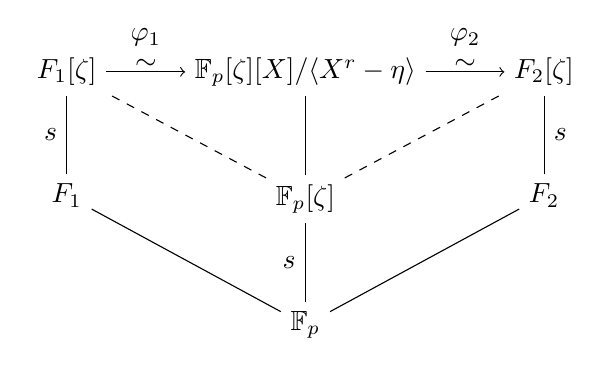
\begin{tikzpicture}
		\node (Fp) {$\F_p$};
		\node[above = of Fp] (Fpz) {$\F_p[\zeta]$};
		\node[above = of Fpz] (Fpzx) {$\F_p[\zeta][X] / \langle X^r - \eta \rangle$};
		\node[left = of Fpzx] (F1z) {$F_1[\zeta]$};
		\node[right = of Fpzx] (F2z) {$F_2[\zeta]$};
		\node[below = of F1z] (F1) {$F_1$};
		\node[below = of F2z] (F2) {$F_2$};
		\draw (Fp) edge (F1) edge (F2) edge node[left, midway] {$s$} (Fpz)
		(Fpz) edge (Fpzx) edge[dashed] (F1z) edge[dashed] (F2z)
		(F1) edge node[left, midway] {$s$} (F1z)
		(F2) edge node[right, midway] {$s$} (F2z);
		\draw[->] (F1z) edge node[above, inner sep=0.5pt] {$ \sim $} node[above = 3mm, inner 
		sep=0.5pt] {$ \varphi_1 $} (Fpzx);
		\draw[->] (Fpzx) edge node[above, inner sep=0.5pt] {$ \sim $} node[above = 3mm, inner 
		sep=0.5pt] {$ \varphi_2 $} (F2z);
		\end{tikzpicture}
		\caption{Constructing isomorphisms}
		\label{figure:isom1}
	\end{center}
\end{figure}





%///////////////////////////////////////////

\subsubsection{Preliminaries}

As mentioned above, we let $s$ be the order of $p$ in $\mathbb{Z} / r\mathbb{Z}$, and write $p^s - 
1 = ur^t$ where $\gcd(r, u) = 1$. The obvious way constructing isomorphisms $\varphi_1, \varphi_2$ 
in Figure \ref{figure:isom1} is to compute an $r$-th root of $\eta$ in $F_1[\zeta], F_2[\zeta]$. 
But, as a more efficient way, we show how to avoid the costly operation of taking roots in these 
extensions, and skip some detail computations. We first need the following result.
\begin{proposition}
	\label{proposition:semi-trace}
	For an element $a \in F_1[\zeta]$ define 
	\begin{equation}
	\label{equation:semi-trace} 
	\theta_a = a + \zeta^{r - 1}a^{p^s} + \cdots + \zeta^2a^{p^{(r - 2)s}} + \zeta a^{p^{(r - 1)s}}
	\end{equation}
	Then
	\begin{enumerate}
		\item[\normalfont (i)] There is an $a \in F_1[\zeta]$ such that $\theta_a \ne 0$.
		\item[\normalfont (ii)] $\theta_a, \theta_a^r$ are non-$r$-adic residues in $F_1[\zeta], 
		\F_p[\zeta]$ respectively.
	\end{enumerate}
\end{proposition}
\begin{proof}
	Let $v = u^{-1} \bmod r$, and let $\gamma \in F_1[\zeta]$ be an $r^t$-th root of $\zeta^{v(r - 
	1)}$. There exists an element $a \in F_1[\zeta]$ such that $\beta = T_{F_1[\zeta] / 
	\F_p[\zeta]}(\gamma a) \ne 0$, and we have 
	\begin{equation}
		\label{equation:trace}
		\begin{aligned}
		\beta 
		& = \gamma a + (\gamma a)^{p^s} + \cdots + (\gamma a)^{p^{(r - 1)s}} \\
		& = \gamma (a + \gamma^{p^s - 1}a^{p^s} + \cdots + \gamma^{p^{(r - 1)s} - 1}a^{p^{(r - 
		1)s}}) \\
		& = \gamma (a + \gamma^{ur^t}a^{p^s} + \cdots + \gamma^{ur^t(p^{(r - 2)s} + \cdots + p^s + 
		1)}a^{p^{(r - 1)s}}) \\
		& = \gamma (a + \zeta^{r - 1}a + \cdots + \zeta a^{p^{(r - 1)s}}) \\
		& = \gamma \theta_a.
		\end{aligned}
	\end{equation}
	This proves (i). To prove (ii), first observe that $\theta_a^{p^s} = \zeta\theta_a$ so that 
	$\sigma(\theta_a) = \zeta\theta_a$ for a generator $\sigma: x \to x^{p^s}$ of $\gal(F_1[\zeta] 
	/ \F_p[\zeta])$. Therefore, we have $\sigma(\theta_a^r) = \theta_a^r$, which means that 
	$\theta_a^r \in \F_p[\zeta]$, and $\theta_a^{ur^t} = \theta_a^{p^s - 1} = \zeta$ which proves 
	that $\theta_a, \theta_a^r$ are non-$r$-adic residues.
\end{proof}
Let $\eta_a = \theta_a^r, \eta_b = \theta_b^r$ for nonzero $\theta_a, \theta_b$ as in Proposition 
\ref{proposition:semi-trace}. Then we can construct isomorphisms $\varphi_1, \varphi_2$ as in the 
following diagram.
\begin{equation}
	\label{equation:iso-chain}
	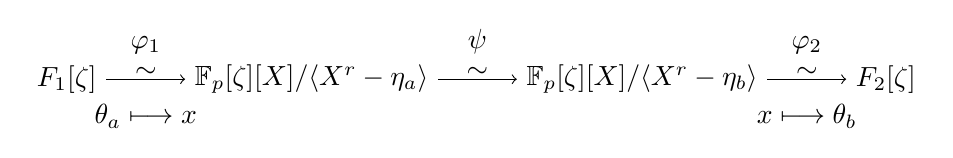
\begin{tikzpicture}
		\node (Fpzxa) {$\F_p[\zeta][X] / \langle X^r - \eta_a \rangle$};
		\node[right = of Fpzxa] (Fpzxb) {$\F_p[\zeta][X] / \langle X^r - \eta_b \rangle$};
		\node[left = of Fpzxa] (F1z) {$F_1[\zeta]$};
		\node[right = of Fpzxb] (F2z) {$F_2[\zeta]$};
		\draw[->] (F1z) edge node[above, inner sep=0.5pt] {$ \sim $} node[above = 3mm, inner 
		sep=0.5pt] {$ \varphi_1 $} node[below = 3mm, inner sep=0.5pt] {$\theta_a \longmapsto x$} 
		(Fpzxa);
		\draw[->] (Fpzxa) edge node[above, inner sep=0.5pt] {$ \sim $} node[above = 3mm, inner 
		sep=0.5pt] {$ \psi $} (Fpzxb);
		\draw[->] (Fpzxb) edge node[above, inner sep=0.5pt] {$ \sim $} node[above = 3mm, inner 
		sep=0.5pt] {$ \varphi_2 $} node[below = 3mm, inner sep=0.5pt] {$x \longmapsto \theta_b$} 
		(F2z);
	\end{tikzpicture}
\end{equation}
To complete this isomorphism chain, we need to compute $\psi$. For that we simply compute an $r$-th 
root of $\eta_a$ in $E = \F_p[\zeta][X] / \langle X^r - \eta_b \rangle$, and construct the 
isomorphism in the obvious way. Note that from (\ref{equation:trace}) we have $\beta_a = 
\gamma_a\theta_a$,  $\beta_b = \gamma_b\theta_b$, and we can choose $\gamma_a, \gamma_b$
such that $\gamma_a^r = \gamma_b^r$. Therefore, 
\[ \eta_a\eta_b^{-1} = \beta_a^r\beta_b^{-r} = (\beta_a\beta_b^{-1})^r = c^r. \] 
So we can construct the isomorphism
\begin{equation*}
	\begin{array}{rrll}
	\psi: & \F_p[\zeta][X] / \langle X^r - \eta_a \rangle & \longrightarrow & \F_p[\zeta][X] / 
	\langle X^r - \eta_b \rangle \\
	& x & \longmapsto & cx
	\end{array}
\end{equation*}
by computing an $r$-th root in $\F_p[\zeta]$.




%///////////////////////////////////////////

\subsubsection{Computing $\theta_a$}

Let $a \in F_1[\zeta]$. To compute $\theta_a$, we use a binary powering scheme similar to the one 
in \cite{doliskanischost2011}. Assuming the representations (\ref{equation:rep}) we let 
\[
\xi_i = x^{p^{is}}, \quad
\delta_i = a + z^{r - 1}a^{p^s} + \cdots + z^2a^{p^{(i - 1)s}} + z^{r - i + 1} a^{p^{(i - 1)s}}.
\]
Then we have the following relations:
\[\xi_1 = x^{p^s}, \quad \delta_1 = a, \]
\[
\xi_i =
\begin{cases}
\xi_{i / 2}^{p^{is / 2}} & \text{if $i$ is even}  \\
\xi_{i - 1}^{p^s} & \text{if $i$ is odd,}
\end{cases} \quad
\delta_i=
\begin{cases}
z^{r - i / 2}\delta_{i / 2}^{p^{is / 2}} + \delta_{i / 2} & \text{if $i$ is even} \\
z^{r - 1}\delta_{i - 1}^{p^s} + \delta_1 & \text{if $i$ is odd}
\end{cases}
\]
Assuming $\xi_i = x^{p^{is}}$ is already known, $\delta_i$ can be computed using the following 
algorithm.

\begin{algorithm}
	[XiDelta$(i, \xi_1,\delta_1)$]
	\label{algorithm:xidelta}
	\begin{algorithmic}[1]
		\REQUIRE a positive integer $i$, $\xi_1 = x^{p^s}$, $\delta_1 = a$
		\ENSURE $\xi_i$, $\delta_i$
		\IF {$i=1$} 
		\RETURN $\xi_1$, $\delta_1$
		\ENDIF
		\STATE $j \leftarrow \lfloor i/2\rfloor$
		\STATE $\xi_{j}, \delta_j \leftarrow {\rm XiDelta}(j,\xi_1,\delta_1)$ 
		\STATE\label{step:xi} $\xi_{2j} \leftarrow \xi_j(\xi_j)$
		\STATE\label{step:delta} $\delta_{2j} \leftarrow z^{r - j}\delta_j(\xi_j) + \delta_j$
		\IF {$i$ is even} 
		\RETURN $\xi_{2j}$, $\delta_{2j}$
		\ENDIF
		\STATE $\xi_i \leftarrow \xi_{2j}(\xi_1)$
		\STATE $\delta_i \leftarrow z^{r - 1}\delta_j(\xi_1) + \delta_1$
		\RETURN $\xi_i$, $\delta_i$
	\end{algorithmic}
\end{algorithm}

\begin{proposition}
	\label{proposition:XiDelta}
	Finding a nonzero $\theta_a$ for random $a \in F_1[\zeta]$ takes \[O(s\CC(r)\log(r) + 
	\MM(r)\log(p))\] operations in $\F_p$.
\end{proposition}
\begin{proof}
	To compute the initial value $\xi_1 = x^{p^s}$ we first compute $x^p$, and then do $\log(s)$ 
	modular compositions at a total cost of $O(\MM(r)\log(p) + C(r)\log(s))$ operations in $\F_p$. 
	Then $\theta_a = \delta_r$ is computed using Algorithm \ref{algorithm:xidelta}: the complexity 
	of the algorithm is dominated by steps \ref{step:xi}, \ref{step:delta}. The former is a
	modular composition in $\F_p[X]$ which takes $C(r)$ operations in $\F_p$. For the later suppose 
	$\delta_j = \delta_{j,0}(x) + \delta_{j,1}(x)z + \cdots + \delta_{j,s - 1}(x)z^{s - 1}$. Then   
	\[ \delta_j(\xi_j) = \sum_{i = 0}^{s - 1}\delta_{ij}(\xi_j)z^i, \] which is done using 
	$O(s\CC(r))$ operations in $\F_p$. Accounting for a recursion depth of $\log(r)$, the running 
	time of the algorithm is then $O(s\CC(r)\log(r))$ operations in $\F_p$. All in all, we get the 
	claimed 
	complexity.
\end{proof}
The above running time for computing $\theta_a$ is only acceptable for small $s$. To keep the 
complexity at most quadratic in $r$ for larger $s$, say $s \in O(r)$, we proceed as follows. We 
know that $T_{F_1[\zeta] / \F_p[\zeta]}(\gamma x^\ell) \ne 0$ for at least one $1 \le \ell \le r - 
1$, otherwise $T_{F_1[\zeta] / \F_p[\zeta]}(\gamma a) = 0$ for all $a \in F_1[\zeta]$ by linearity.
Therefore, the linear map 
\[
\begin{array}{rrll}
	T_{F_1[\zeta] / \F_p[\zeta]}\vert_{F_1}: & F_1 & \longrightarrow & \F_p[\zeta] \\
	& d(x) & \longmapsto & T_{F_1[\zeta] / \F_p[\zeta]}(\gamma d(x))
\end{array}
\]
is not identically zero. This implies that we need to try at most $O(1)$ random $d(x) \in F_1$ to 
obtain a nonzero
\[ \theta_{d(x)} = d(x) + \zeta^{r - 1}d(x)^{p^s} + \cdots + \zeta^2d(x)^{p^{(r - 2)s}} + \zeta 
d(x)^{p^{(r - 1)s}}. \]
The sequence $d(x), d(x)^{p^s}, \dots, d(x)^{p^{(r - 1)s}}$ in $F_1$ can be computed by Algorithm 
3.1 in \cite{von1992computing} using $O(\MM(r^2)\log(r))$ operations in $\F_p$. Therefore, we have 
proved the following,
\begin{proposition}
	\label{proposition:XiDelta-updated}
	Finding a nonzero $\theta_a$ for random $a \in F_1[\zeta]$ takes
	\begin{itemize}
		\item $O(s\CC(r)\log(r) + \MM(r)\log(p))$ operations in $\F_p$ for small $s$, or
		\item $O(\MM(r^2)\log(r) + \MM(r)\log(p))$ operations in $\F_p$ for large $s$.
	\end{itemize}
\end{proposition}



%///////////////////////////////////////////

\subsubsection{Computing $r$-th roots in $\F_p[\zeta]$}
\label{subsection:rth-root-fpz}

Let $a \in \F_p[\zeta]$ be an $r$-th power. To compute an $r$-th root of $a$ we factor the 
polynomial $X^r - a$ using the Equal Degree Factorization algorithm given in 
\cite{kaltofen+shoup97}.
\begin{algorithm}
	[Root Finding]
	\label{algorithm:edf}
	\begin{algorithmic}[1]
		\REQUIRE a square-free polynomial $f \in \F_p[\zeta][x]$ of degree $n$ with linear factors
		\ENSURE a single factor of $f$
		\IF {$\deg f = 1$}
		\RETURN $f$
		\ENDIF
		\STATE Pick a random element $\alpha \in \mathbb{A}_f = \F_p[\zeta][x]/\langle f \rangle$
		\STATE\label{step:edf-trace} Compute the following trace in $\mathbb{A}_f$
		\[ \beta = \alpha + \alpha^p + \alpha^{p^2} + \cdots + \alpha^{p^{s - 1}} \]
		\STATE $\gamma \leftarrow \beta^{(p - 1) / 2}$
		\STATE $g \leftarrow \gamma \bmod f$, $g_1 \leftarrow \gcd(g, f)$, $g_2 \leftarrow \gcd(1 + 
		g, f)$
		\STATE Recursively factor one of $g_1, g_2$ that is non-constant
	\end{algorithmic}
\end{algorithm}
The dominant cost of the algorithm comes from Step \ref{step:edf-trace}, which is done as follows. 
Let
\[ \beta_i = \alpha^p + \alpha^{p^2} + \cdots + \alpha^{p^i}, \quad \xi_i = x^{p^i}, \quad \zeta_i 
= z^{p^i}. \]
Then we have $\beta_1 = \alpha^p$, $\xi_1 = x^p$, $\zeta_1 = z^p$, and
\[
\beta_j = 
\begin{cases}
	\beta_{j / 2} + \beta_{j / 2}^{p^{j / 2}} & j \text{ even} \\
	\beta_1 + \beta_{j - 1}^p & j \text{ odd}
\end{cases}, \quad
\xi_j = 
\begin{cases}
	\xi_{j / 2}^{p^{j / 2}} & j \text{ even} \\
	\xi_{j - 1}^p & j \text{ odd}
\end{cases}, \quad
\zeta_j = 
\begin{cases}
	\zeta_{j / 2}^{p^{j / 2}} & j \text{ even} \\
	\zeta_{j - 1}^p & j \text{ odd}
\end{cases}
\]
For a positive integer $j$ we have
\begin{equation}
	\label{equation:betaj}
	\beta_j^{p^j} = \left( \sum_{l = 0}^{n - 1}c_l(z)x^l \right)^{p^j} = \sum_{l = 0}^{n - 
	1}c_l(z^{p^j})(x^{p^j})^l = \sum_{l = 0}^{n - 1}c_l(\zeta_j)\xi_j^l.
\end{equation}
Therefore we have a recursive algorithm for computing $\beta = \beta_{s - 1}$. Let us analyze the 
complexity of the algorithm. First note that we always have $z^r = 1, x^r = a$. This makes it 
possible to keep the identities simple and do the reductions at the end of each step. For example 
$x^p = a^{\lfloor p / r\rfloor}x^{p \bmod r}$ which can be computed using $O(\MM(s)\log(p))$
operations in $\F_p$. At step $j$ of the recursion we have the following costs in $\F_p$:
\begin{itemize}
	\item $O(\MM(r) + \MM(s)\log(r))$ for computing $x^{p^j}$, and computing $z^{p^j}$ is free.
	\item If $s$ is small we can first reduce $z^{p^j \bmod r}$ modulo $g(Z)$, and then do $n$ 
	modular compositions at a total cost
	of $O(\MM(r) + n\CC(s))$. But if $s$ is large we can reduce $c_l(z^{p^j \bmod r})$ modulo 
	$g(Z)$ for all $0 \le l < n$ at a total cost of $O(n\MM(r))$.
	\item $O(n\MM(s))$ for evaluating $\beta_j$ at $x^{p^j}$ using Horner's method.
	\item $O(\MM(r)\MM(s))$ for reducing (\ref{equation:betaj}) modulo $f$.
\end{itemize}
The depth of the recursion is $\log(s)$, hence $\beta$ can be computed in
\begin{itemize}
	\item $O(\MM(s)\log(p) + n\CC(s)\log(s) + \MM(r)\MM(s)\log(s))$ operations in $\F_p$ for small 
	$s$, or
	\item $O(\MM(s)\log(p) + n\MM(r)\log(s) + \MM(r)\MM(s)\log(s))$ operations in $\F_p$ for large 
	$s$.
\end{itemize} 
Finally since the depth of the recursion in Algorithm \ref{algorithm:edf} is $\log(r)$, we have the 
following.
\begin{proposition}
	\label{proposition:root-fpz}
	The total cost of root finding in $\F_p[\zeta]$ is
	\begin{itemize}
		\item $O(\MM(s)\log(p)\log(r) + r\CC(s)\log(s) + \MM(r)\MM(s)\log(s)\log(r))$\\ operations 
		in 
		$\F_p$ for small $s$, or
		\item $O(\MM(s)\log(p)\log(r) + r\MM(r)\log(s) + \MM(r)\MM(s)\log(s)\log(r))$\\ operations 
		in 
		$\F_p$ for large $s$.
	\end{itemize}
\end{proposition}





%///////////////////////////////////////////

\subsubsection{Computing the isomorphism $F_1 \rightarrow F_2$}

In this section, we analyze the computational cost of building an isomorphism $\varphi: F_1 
\rightarrow F_2$. We first construct the isomorphism $\varphi_2 \circ \psi \circ \varphi_1 : 
F_1[\zeta] \rightarrow F_2[\zeta]$ as in (\ref{equation:iso-chain}), and then descend back to the 
desired fields. The following algorithm builds the above chain of isomorphism based on the 
observations at the start of the section. 
\begin{algorithm}
	[Isomorphism ${F_1[\zeta] \rightarrow F_2[\zeta]}$]
	\label{algorithm:ext-iso}
	\begin{algorithmic}[1]
		\REQUIRE degree $r$ extensions $F_1, F_2$ of $\F_p$
		\ENSURE an isomorphism $F_1[\zeta] \rightarrow F_2[\zeta]$
		\STATE\label{step:factor-cyclo} factor the cyclotomic polynomial $\Phi_r(Z)$ over $\F_p$ to 
		build extensions $\F_p[\zeta],
		F_1[\zeta], F_2[\zeta]$
		\REPEAT
		\STATE choose a random $a \in F_1[\zeta]$
		\STATE compute $\theta_a$ using Algorithm \ref{algorithm:xidelta}
		\UNTIL {$\theta_a \ne 0$}
		\REPEAT
		\STATE choose a random $b \in F_2[\zeta]$
		\STATE compute $\theta_b$ using Algorithm \ref{algorithm:xidelta}
		\UNTIL {$\theta_b \ne 0$}
		\STATE\label{step:gamma-pow} $\eta_a \leftarrow \theta_a^r$ , $\eta_b \leftarrow \theta_b^r$
		\STATE\label{step:psi} construct the isomorphism $\psi$ as in (\ref{equation:iso-chain})
		\STATE construct $F_1[\zeta] \rightarrow F_2[\zeta]$ as in (\ref{equation:iso-chain})
	\end{algorithmic}
\end{algorithm}
\begin{proposition}
	Algorithm \ref{algorithm:ext-iso} computes the isomorphism $F_1[\zeta] \rightarrow F_2[\zeta]$ 
	using
	\begin{itemize}
		\item $O(s\CC(r)\log(r) + \MM(r)\log(p) + \MM(s)\log(p)\log(r))$\\ operations in $\F_p$ for 
		small $s$, or
		\item $O(\MM(r)\log(p) + \MM(s)\log(p)\log(r) + \MM(r^2)\log(r) + 
		\MM(s)\MM(r)\log(s)\log(r))$\\ 
		operations in $\F_p$ for large $s$.
	\end{itemize}
\end{proposition}
\begin{proof}
	By \cite[Theorem 9]{shoup94} Step \ref{step:factor-cyclo} takes $O(r\log^2(r) + 
	r\log(r)\log(p))$ operations in $\F_p$. The running time of the two repeat...until loops is 
	given by Proposition \ref{proposition:XiDelta-updated}. Step \ref{step:gamma-pow}
	is done using $O(\MM(s)\MM(r)\log(r))$ operations in $\F_p$. The running time of Step 
	\ref{step:psi} is given by Proposition \ref{proposition:root-fpz}. Adding all these up proves 
	the proposition.
\end{proof}
So, now we have an isomorphism $\phi: F_1[\zeta] \rightarrow F_2[\zeta]$ that sends $\theta_a$ to 
some $h(z, x) \in F_2[\zeta]$. To construct the isomorphism $\varphi: F_1 \rightarrow F_2$ we the 
technique in \cite{Allombert02}. Let 
\[ \theta_a = \sum_{i = 0}^{s - 1}f_i(x)z^i, \quad\text{and}\quad z^s = (v(z)  \bmod g(z)) = 
\sum_{i = 0}^{s - 1}v_iz^i. \] 
Then since $\theta_a^{p^s} = z\theta_a$ we have
\[ \sum_{i = 0}^{s - 1}f_i(x)^{p^s}z^i = f_{s - 1}(x)v(z) + f_0(x)z + \cdots + f_{s - 2}(x)z^{s - 
1}.\]
After rearranging the terms in the right hand side, this gives us the identities
\[
\begin{array}{ccc}
	f_0(x)^{p^s} & = & v_0f_{s - 1}(x) \\
	f_1(x)^{p^s} & = & f_0(x) + v_1f_{s - 1}(x) \\
	\vdots & \vdots & \vdots \\
	f_{s - 1}(x)^{p^s} & = & f_{s - 2}(x) + v_{s - 1}f_{s - 1}(x)
\end{array} 
\]
form which we see that $f_i(x) \in \F_p(f_0(x)) \subseteq F_1$ for all $i$. We prove $\F_p(f_0) = 
F_1$. Let $\sigma \in \gal(F_1(z) / \F_p)$ be a generator, and let $j \le r$ be the smallest 
integer such that $\sigma^jf_0 = f_0$. Then $\sigma^{js}\theta_a = \theta_a$, but $\theta_a$ is not 
contained in any proper subfield; so $j = r$. Let $h_0$ be the constant term of $h(z, x)$. Then we 
similarly have $F_2 = \F_p(h_0)$. This gives us an isomorphism
\[
\begin{array}{rlll}
	\phi: & F_1 & \longrightarrow & F_2 \\
	& f_0 & \longmapsto & h_0
\end{array}
\]
from which we can get an isomorphism
\[
\begin{array}{rlll}
	\phi: & F_1 & \longrightarrow & F_2 \\
	& x & \longmapsto & a(x)
\end{array}
\]
using transposed modular composition.


%%%%%%%%%%%%%%%%%%%%%%%%%%%%%%%%%%
\section{Rains' algorithm}

In his paper, Pinch \cite{} proposed to use specific generating element to solve
the isomorphism problem. One of his two methods makes use of the cyclotomic
extension.\par
Let $\F_q$ be a finite field of characteristic $p$ and let $n$ be an integer. 
Now, let $m$ be an integer such that the primitive $m$th roots span 
$\F(q^n)$, and let $f$ and $g$ be two different irreducible polynomial of
degree $n$ over $\F_q$. We note
\begin{equation}
k_1 := \F_q[X]/(f)\text{ and }k_2 := \F_q[X]/(g)
\end{equation}
Pinch's method consists of finding primitive $m$th roots of unity in both extensions
$k_1$ and $k_2$, which we will called $\alpha$ and $\beta$ respectively, then
find the morphism
\begin{equation}
\varphi_e : \alpha\longmapsto\beta^e
\end{equation}
which actually defines an isomorphism.\par
One of the issue with this method is that the order of $\F(q^n)$ may only be
divisible by large integers, increasing drastically the time it takes to find a 
$m$th root of unity in each extensions. Another issue is the random choice of
primitive $m$th roots. Due to how the cyclotomic polynomial factors in
charateristic $p$, it could take $O(m)$ tries to find two roots which are not in
the same irreducible factor.\par

\subsection{Gaussian periods}

A solution to the problem mentionned above would be to find a way to generate
elements which define an isomorphism. Those elements are the \emph{Gaussian
periods} that will be introduced in this section.\par
Let $L$ be a number fields of degree $\ell$ and $\mathcal{O}_{K}$ its ring of
integers. Let $q = p^{\ell}$ and $\mu_m$ be the abstract group of $m$th roots of
unity. If we let $\mathfrak{p}$ be the ideal of $L$ above $p$ such that
$\mathcal{O}_L/\mathfrak{p} = \F_q$ and $\mathfrak{P}$ one of its irreducible 
factors in $L[\mu_m]$, we have the following situation.


\begin{center}
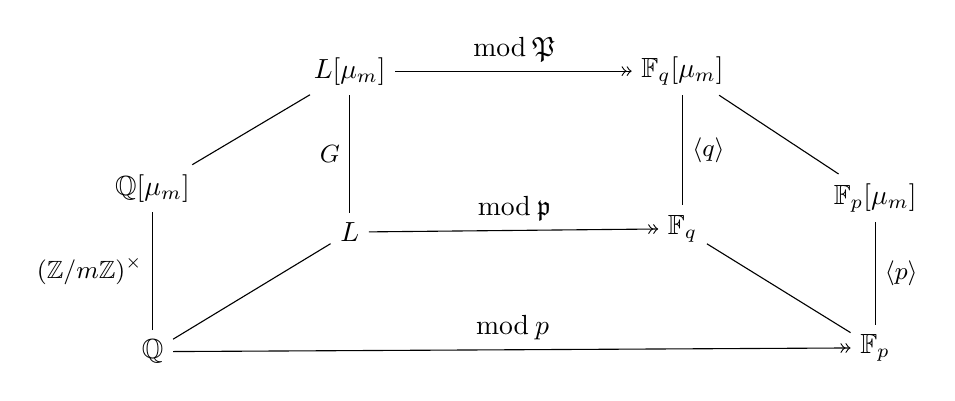
\begin{tikzpicture}
    \node (Q) {$\Q$};
    \node[above =1.5cm of Q] (Qm) {$\Q[\mu_m]$};
    \node[above right=1cm and 2cm of Q] (L) {$L$};
    \node[above =1.5cm of L] (Lm) {$L[\mu_m]$};
    \node[right =3cm of Lm] (Fqm) {$\F_q[\mu_m]$};
    \node[below =1.4cm of Fqm] (Fq) {$\F_q$};
    \node[below right=1cm and 1.15cm of Fqm] (Fpm) {$\F_p[\mu_m]$};
    \node[below =1.3cm of Fpm] (Fp) {$\F_p$};
    \draw (Q) edge node[left] {\small $(\Z/m\Z)^{\times}$} (Qm); 
    \draw (L) edge node[left] {\small $G$} (Lm); 
    \draw (Fqm) edge node[right] {\small $\langle{q}\rangle$} (Fq); 
    \draw (Fpm) edge node[right] {\small $\langle{p}\rangle$} (Fp); 
    \draw (Q) edge node {} (L);
    \draw (Qm) edge node {} (Lm);
    \draw (Fqm) edge node {} (Fpm);
    \draw (Fq) edge node {} (Fp);
    \draw[->>] (Q) edge node[above] {$\bmod\, p$} (Fp);
    \draw[->>] (L) edge node[above] {$\bmod\, \mathfrak{p}$} (Fq);
    \draw[->>] (Lm) edge node[above] {$\bmod\, \mathfrak{P}$} (Fqm);
\end{tikzpicture}
\end{center}

where $G$ is the Galois group of $L[\mu_m]/L$ subgroup of $(\Z/m\Z)^{\times}$
and $\langle{q}\rangle$, $\langle{p}\rangle$ are the decomposition groups of
$\mathfrak{P}/\mathfrak{p}$ and $\mathfrak{p}/p$ respectively.

\begin{definition}
Let us assume that there exists a subgroup $S\subset(\Z/m\Z)^{\times}$ such that
\begin{equation}
(\Z/m\Z)^{\times} = \langle{q}\rangle \times S.
\end{equation}
Then for every generator $\zeta_m$ of $\mu_m$, we define the Gauss periods
$\eta(\zeta_m)$ as follow
\begin{equation}
\eta(\zeta_m) = \sum_{\sigma\in S}{\zeta_m^{\sigma}}.
\end{equation}
\end{definition}

\subsection{Rains' special algorithm}

\subsection{Rains' cyclotomic algorithm}

\subsection{Complexity analysis}


%%%%%%%%%%%%%%%%%%%%%%%%%%%%%%%%%%

\section{Elliptic Rains' algorithm}

In \cite{}, Pinch already proposed to use the torsion point of an elliptic
curve in place of the roots of unity. Rains also mentionned this possiblity, 
but judges that as far as he could see it would not bring significant 
improvements.\par 
In practice the use of auxiliary extensions in the cyclotomic method costs a of
ressources.We will see that, contrary to Rains' belief, in the cases where an
auxiliary extention is necessary, the elliptic variant is actually more 
competitive.\par
In the next sections, we will first introduce the \emph{elliptic periods} which 
plays a similar role as the Gaussian periods, then we will describe the
algorithm itself and finally we will compute its complexity; which will
roughly be $\tildO(n^2)$ just like the other variants, the difference will be 
on the constant of the big $O$.

\subsection{Elliptic periods}

The use of elliptic curve raises another kind of problem that was not present 
in the cyclotomic version of Rains' algorithm. The fact is elliptic curves 
come with non trivial automorphisms that can't be ignored. This will be taken 
in account in the definition of the elliptic periods. In particular, the cases 
$j = 0, 1728$ shall be dealt more specifically.\par
As in the
previous sections, we work in positive charactestic $p$, with the addition of
$p \neq 2$ or $3$, we denote by $f$ and $g$ two disctinct irreducible
polynomials of degree $n$ on $\F_q$ and we let $k_1$ and $k_2$ be the
respective extensions they define. Let us quickly recall the definition of an 
Elkies Prime. 

\begin{definition}
Let $E/\F_q$ be an elliptic curve, let $m$ be a prime, we say that $m$
is an Elkies prime for $E$ if the charateristic polynomial of its Frobenius
$\pi_q : (X, Y, Z) \to (X^q, Y^q, Z^q)$ splits in $\Z/m\Z$, in other words
\begin{equation}
X^2 - tX + q = (X - a)(X - b) \bmod m
\end{equation}
for $a,b\in\Z/m\Z$ and $t$ the trace of the Frobenius $\pi_q$ such that 
$\# E(\F_q) = q + 1 - t$.
\end{definition}

\begin{remark}
\emph{note : à retravailler}\\
If $m$ is an Elkies prime for $E$, then there exists a basis such that the 
Frobenius acts as a diagonale matrix on $E[m]$, on which the restriction of
$\pi$ is decomposed in two eigenspaces; the eigenvalues are the root of the 
characteristic polynomial of the Frobenius :
\begin{equation}
\begin{pmatrix}
a & 0\\
0 & b
\end{pmatrix}.
\end{equation}
For all integer $n$, the action Frobenius of $E/\F_{q^n}$ will be the $n$th
power of that matrix. Additionnaly, if you note $k =
\textup{min}(\order_m(a),\order_m(b))$ then the extension $\F_{q^k}$ is
the smallest extension on which there is a torsion point. Let $k = \order_m(a)$
and $P$ be in the eigenspace of $a$, then we have the following
\begin{equation}
\pi_{q^k}(P) = [a^k]P = [1] = P
\end{equation}
Moreover, this also show that with good conditions the abscissas of points in the 
eigenspace of $a$ generates $\F_{q^k}$. This will be used in the next
section.
\end{remark}

\begin{definition}
Let $E/\F_q$ be an elliptic curve and let $m>2$ be an Elkies prime for $E$.\par
\begin{itemize}
\item Let us consider the case where $j\neq0, 1728$. Let $a$ be
an eigenvalue of $\phi_q \bmod m$. Suppose there exists a subgroup $S$ of
$(\Z/m\Z)^{\times}$ such that 
\begin{equation}
(\Z/m\Z)^{\times}/\lbrace{\pm1}\rbrace = \langle{a}\rangle \times S
\end{equation}
Then for every $P\in E[m]$ in the eigenspace generated by $a$, we define
the elliptic periods as follow
\begin{equation}
\eta_{a}(P) = \sum_{\sigma\in S}{\left([\sigma]P\right)_X}
\end{equation}
where $P_X$ denotes the abscissa of the point $P$.\par
     
\item For the cases $j = 0$ or $1728$, we have to take in account the size
of $\Aut_{\F_q}(E)$. Namely, we shall assume that its order divides $\varphi(m)$
then we identify it to a subgroupe of $(\Z/m\Z)^{\times}$. We once again assume
that there is a subgroup $S$ of $(\Z/m\Z)^{\times}$ such that
\begin{equation}
(\Z/m\Z)^{\times}/\Aut_{\F_q}(E) = \langle{a}\rangle\times S
\end{equation}
Then for every $P\in E[m]$ in the eigenspace generated by $a$, we define
the elliptic periods as follow
\begin{equation}
\eta_{a}(P) = \sum_{\sigma\in
S}{\left([\sigma]P\right)_X^{\#\Aut_{\F_q}(E)/2}}
\end{equation}\par
\end{itemize}

\end{definition}

Notice that the first description is a particular case of the last definition.
As we noted earlier, the elliptic periods will play the same role as the
Gaussian periods in the cyclotomic variant. We shall now enounce the main
theorem of this section.

\begin{theorem}
\label{theorem:ellperiods}
Let $m$ be a prime different from $p$ and $t$ an integer such that 

\begin{enumerate}

    \item $\mid t\mid < \sqrt{2q}$,
    \item $X^2 - tX + q = (X - a)(X - b)\bmod m,$
    \item $(\Z/m\Z)^{\times}/\Aut_{\F_q}(E) = \langle{a}\rangle \times S$ for $S$ a subgroup of
$(\Z/m\Z)^{\times}$,
    \item $\order_m(a) = n$ and $\order_m(b) \nmid n$.
\end{enumerate}
Now, let $E/\F_q$ be an elliptic curve of trace $t$. Then $\F_{q^n}$ is the
smallest extension that contains $m$-torsion points and for all $P$ in the
eigenspace of $a$, the periods $\eta_a(P)$ form a normal basis of $\F_{q^n}$ on
$\F_q$.

\end{theorem}

To prove this theoreme, we will have to move back to characteristic $0$ just
like in the previous section.

\subsection{Elliptic algorithm}

The main improvement of the elliptic variant of Rains' algorithm is the fact
that we can work directly in the extensions we are interested in. What allows
this to happen is that contrary to the roots of unity, there isn't only one
elliptic curve per extension, namely there are as many elliptic curves as there
are $j$-invariants in $\F_q$. Even more so, the use of twist of curves, which we
will be talking about later, ensures to almost always find the elliptic curve we
need for our algorithm.\\\par

\subsubsection*{Finding an elliptic curve}
If theoritically, we always introduce the elliptic curve before finding an
Elkies prime number, in practice, we have to find a prime $m$ which has the good
properties and then we pick an elliptic curve for which this $m$ is an Elkies
prime.\par
At first, we will concentrate on $p\neq2,3$. We need to find an integer $m$ 
such that there exist an element of order $n$ modulo $m$, so that the first 
extension on which there will be rational torsion point of order $m$ is 
$\F_{q^n}$. The first condition is then $n\mid \varphi(m)$. We also require 
that the cofactor $\varphi(n)/n$ is prime with $n$, so it ensures that the right 
groups split as we want, namely 
\begin{equation}
(\Z/m\Z)^{\times}/\Aut_{\F_q}(E)=\langle{a}\rangle\times S
\end{equation}
for $S$ a subgroup of $(\Z/m\Z)^{\times}$ and $a$ the eigenvalue of $\pi_q$ of
order $n$ modulo $m$. We also wish for $b$, the other eigenvalue of $\pi_q$ to
be of order not dividing $n$, because...\par
To pick a good elliptic curve, we shall first pick some trace candidate modulo 
$m$. Since we need $m$ to be an Elkies prime for the future elliptic curve, the
polynomial in $(\Z/m\Z)$ shall be of the form
\begin{equation}
(X - a)(X - b) = X^2 - (a + b)X + ab \bmod m.
\end{equation}
Then we pick $a\in(\Z/m\Z)^{\times}$ such that $\order_m(a) = n$ and,
since $ab = q$, we check that $\order_m(a/q)\nmid n$. If these conditions are
met, we note $t = a + a/q \bmod m$ and check if it is a good trace candidate
using Hasse theorem. More precisely, we verify that $\hat{t}$ the lift of $t$ is
actually in the Hasse's bound
\begin{equation}
|\hat{t}| \leq 2\sqrt{q}.
\end{equation}\\\par
To chose the right elliptic curve, we pick a $j\in\F_q$ and compute the trace of
the associated ellpitic curve to check if it is equal to one of the candidates
we picked previously. Before testing the curves for other $j$-invariant, should
the trace not be a match for any candidate, it is important to know that there
are serveral curves defined for one $j$-invariant; these are called twists of an
elliptic curve. We will use a proposition from \cite{Silverman} as a
definition.

\begin{definition}
Let $E/\F_q$ be an elliptic curve and let $A,B\in\F_q$ be such that
\begin{equation}
E : y^2 = x^3 + AX + B
\end{equation}
is its Weierstrass equation. Then for $D\in(\F_q)^*$ we define the twist $E_D$
of $E$ corresponding to $D$ as follow.

\begin{equation*}
\begin{aligned}
(i)\quad & E_D : y^2 = x^3 + D^2Ax + D^3B && \text{if } j(E)\neq0,1728,\\
(ii)\quad & E_D : y^2 = x^3 + DAx && \text{if } j(E)=1728,\\
(iii)\quad & E_D : y^2 = x^3 + DB && \text{if } j(E)=0.
\end{aligned}
\end{equation*}

\end{definition}

\begin{remark}
For $j\neq0,1728$, the twist is called a quadratic twist and for it to be
different from $E$, $D$ needs to be a non-quadratic residue. For $j=1728$, $D$
needs to be a non-quadratic residue and for $j = 0$, $D$ needs to be a
non-cubic residue as well. The twists are called quartic twists and sextic twists
respectively.
\end{remark}

We can deduce quite simply that the trace of quadratic twist is the
opposite of the original curve. TODO\par
There are similar results for the other $j$-invariant which will be detailed in
the next proposition.

\begin{proposition}
\label{proposition:twisttrace}
Let $E/\F_q$ be an ordinary elliptic curve and $j_E$ its $j$-invariant. We have
one of the following.

\begin{enumerate}
    \item For $j_E\neq0,1728$, we let $D\in\F_q$ be a non-quadratic residue, then
the trace of the quadratic twist $E_D$ of $E$ satisfies the relation
\begin{equation}
t_{E_D} = -t_E.
\end{equation}

    \item For $j_E=1728$ and $q=1\bmod4$, we let $D\in\F_q$ be a non-quadratic residue, then the
traces of the quartic twists $E_D$ of $E$ statisfy
\begin{equation}
t_{E_D} = \zeta_4t_E,
\end{equation}
for $\zeta_4\in\F_q$ a $4th$ root of unity.

    \item For $j_E=0$ and $q=1\bmod6$, we let $D\in\F_q$ be a non-quadratic
residue and a non-cubic residue, then the
traces of the sextic twists $E_D$ of $E$ statisfy
\begin{equation}
t_{E_D} = \zeta_6t_E,
\end{equation}
for $\zeta_6\in\F_q$ a $6th$ root of unity.
\end{enumerate}

\end{proposition}

\begin{proof}
\end{proof}

In summary, we need to find an integer $m$ such that :
\begin{itemize}
    \item $m$ is prime,
    \item $n\mid\varphi(m)$ and $(\varphi(m)/n,n)=1$,
    \item there exists $a\in(\Z/m\Z)^{\times}$ such that 
\begin{equation}
\label{equation:ordeigen}
\order_m(a) = n,\order_m(\dfrac{a}{q}) \nmid n\text{ and }|\widehat{a + \dfrac{a}{q}}| \leq 2\sqrt{q}.
\end{equation}
\end{itemize}
Let
\begin{equation}
\mathcal{T}_m = \lbrace{t = a + a/q \bmod m \text{ with } a\in(\Z/m\Z)^{\times}
\text{ such that } a \text{ satisfies 
}(\ref{equation:ordeigen})}\rbrace
\end{equation}
the good trace candidates for a prime $m$, then the
routine to find a good elliptic curve is as follow.

\begin{algorithm}
    [Selecting an elliptic curve]
    \label{algorithm:selectell}
    \begin{algorithmic}[1]
    \REQUIRE $m$ an integer as above, $q$ a prime power, $n$ the extension
degree, $\mathcal{T}_m$, $c$ a generator of $(\Z/m\Z)^{\times}$
    \ENSURE $E$ an elliptic curve with $t_E\in\mathcal{T}_m$
    \STATE $E\leftarrow \text{EllipticCurve}(j=1728)$
    \STATE $t_E\leftarrow \text{Trace}(E)$
    \IF{$q\neq1\bmod4$ \AND $0\in\mathcal{T}_m$}
        \RETURN $E$
    \ELSE
        \FOR{$i\in\lbrace{0,\dots,3}\rbrace$}
            \IF{$\zeta_4^it_E\in\mathcal{T}_m$}
                \RETURN $\text{quartic\_twist}(E,c^i)$
            \ENDIF
        \ENDFOR
    \ENDIF
    \STATE $E\leftarrow \text{EllipticCurve}(j=0)$
    \STATE $t_E\leftarrow \text{Trace}(E)$
    \IF{$q\neq1\bmod6$ \AND $0\in\mathcal{T}_m$}
        \RETURN $E$
    \ELSE
        \FOR{$i\in\lbrace{0,\dots,5}\rbrace$}
            \IF{$\zeta_6^it_E\in\mathcal{T}_m$}
                \RETURN $\text{sextic\_twist}(E,c^i)$
            \ENDIF
        \ENDFOR
    \ENDIF
    \FOR{$j_0\in\F_q$ \AND $j_0\neq0,1728$}
        \STATE $E\leftarrow \text{EllipticCurve}(j=j_0)$
        \STATE $t_E \leftarrow \text{Trace}(E)$
        \FOR{$\zeta\in\lbrace{1,-1}\rbrace$}
            \IF{$\zeta t_E\in\mathcal{T}_m$}
                \RETURN $\text{quadratic\_twist}(E)$
            \ENDIF
        \ENDFOR
    \ENDFOR
    \end{algorithmic}
\end{algorithm}

\subsubsection*{Computing the elliptic periods}

Computing the elliptic periods isn't the most complicated part of the algorithm.
Counting the points of $E/\F_{q^n}$ is directly deduced from the number of
points of $E/\F_q$ using the relation
\begin{equation}
\# E(\F_q^n) = q^n + 1 - (a^n + b^n)
\end{equation}
for $a, b$ the roots of the characteristic polynomial of $\pi_q$. To find a
point of order $m$ in the eigenspace of $a$, we just have to find a point of
order $m$ in $\F_{q^n}$ thanks to the properties on the order of the eigenvalue.

\subsection{Complexity analysis}

\section{Experimental Results}

%%%%%%%%%%%%%%%%%%%%%%%%%%%%%%%%%%
%%%%%%%%%%%%%%%%%%%%%%%%%%%%%%%%%%

\part{Embedding evaluation}

%%%%%%%%%%%%%%%%%%%%%%%%%%%%%%%%%%

\section{Algorithms specific to normal bases}

%%%%%%%%%%%%%%%%%%%%%%%%%%%%%%%%%%

\section{Monomial-dual bases pairs}

%%%%%%%%%%%%%%%%%%%%%%%%%%%%%%%%%%

\section{Experimental results}

%%%%%%%%%%%%%%%%%%%%%%%%%%%%%%%%%%

\section{Conclusion}

%%%%%%%%%%%%%%%%%%%%%%%%%%%%%%%%%%
%%%%%%%%%%%%%%%%%%%%%%%%%%%%%%%%%%

\bibliographystyle{plain}
\bibliography{defeo}

\end{document}


% Local Variables:
% ispell-local-dictionary:"american"
% End:

%  LocalWords:  isomorphism
